\section{问题四：救援任务分区与资源配置优化}
\label{sec:q4}

\subsection{问题分析与关键规则形式化}

问题四要求把 15 个服务区划分为 2 组与 3 组两种任务分区方案，并核算每组\textbf{独立执行}所需的四类资源。其关键规则有两条：

\begin{itemize}[leftmargin=2em]
	\item \textbf{刚性继承}：必须保持问题三已确定的货箱组批、服务区访问顺序、运输与中继任务安排、通信保障关系\textbf{不变}；
	\item \textbf{同架次同组}：若同一运输架次同时涉及多个服务区，则这些服务区\textbf{必须划入同一任务组}。
\end{itemize}

第二条规则是本题的建模关键。它在服务区之间建立了一个\textbf{等价关系}：同一架次所访问的服务区两两"必须同组"。把所有此类约束求并，即得到服务区集合上的一个等价关系，其等价类正是该关系诱导的\textbf{连通分量}\cite{lari2015connectedpartition}。因此，任务分区问题自然地建模为\textbf{图与连通分量}问题：

\begin{itemize}[leftmargin=2em]
	\item 以 15 个服务区为顶点；若两个服务区出现在同一运输架次中，则连一条边；
	\item 每个\textbf{连通分量}是一个\textbf{原子单元}——单元内的服务区不可被拆到不同任务组；
	\item 合法的 $K$ 组分区存在，当且仅当该图可以被划分为 $K$ 个连通分量（即 $K\le$ 原子单元数）。
\end{itemize}

\subsection{连通分量分析与分区可行性}

\textbf{（1）构图。}对问题三方案的 16 个运输架次构图。其中 \textbf{12 个为访问 $\ge2$ 个服务区的多点架次}，这些架次把原本孤立的服务区连接起来。所得关联图如图~\ref{fig:q4_graph} 所示。

\begin{figure}[htbp]
	\centering
	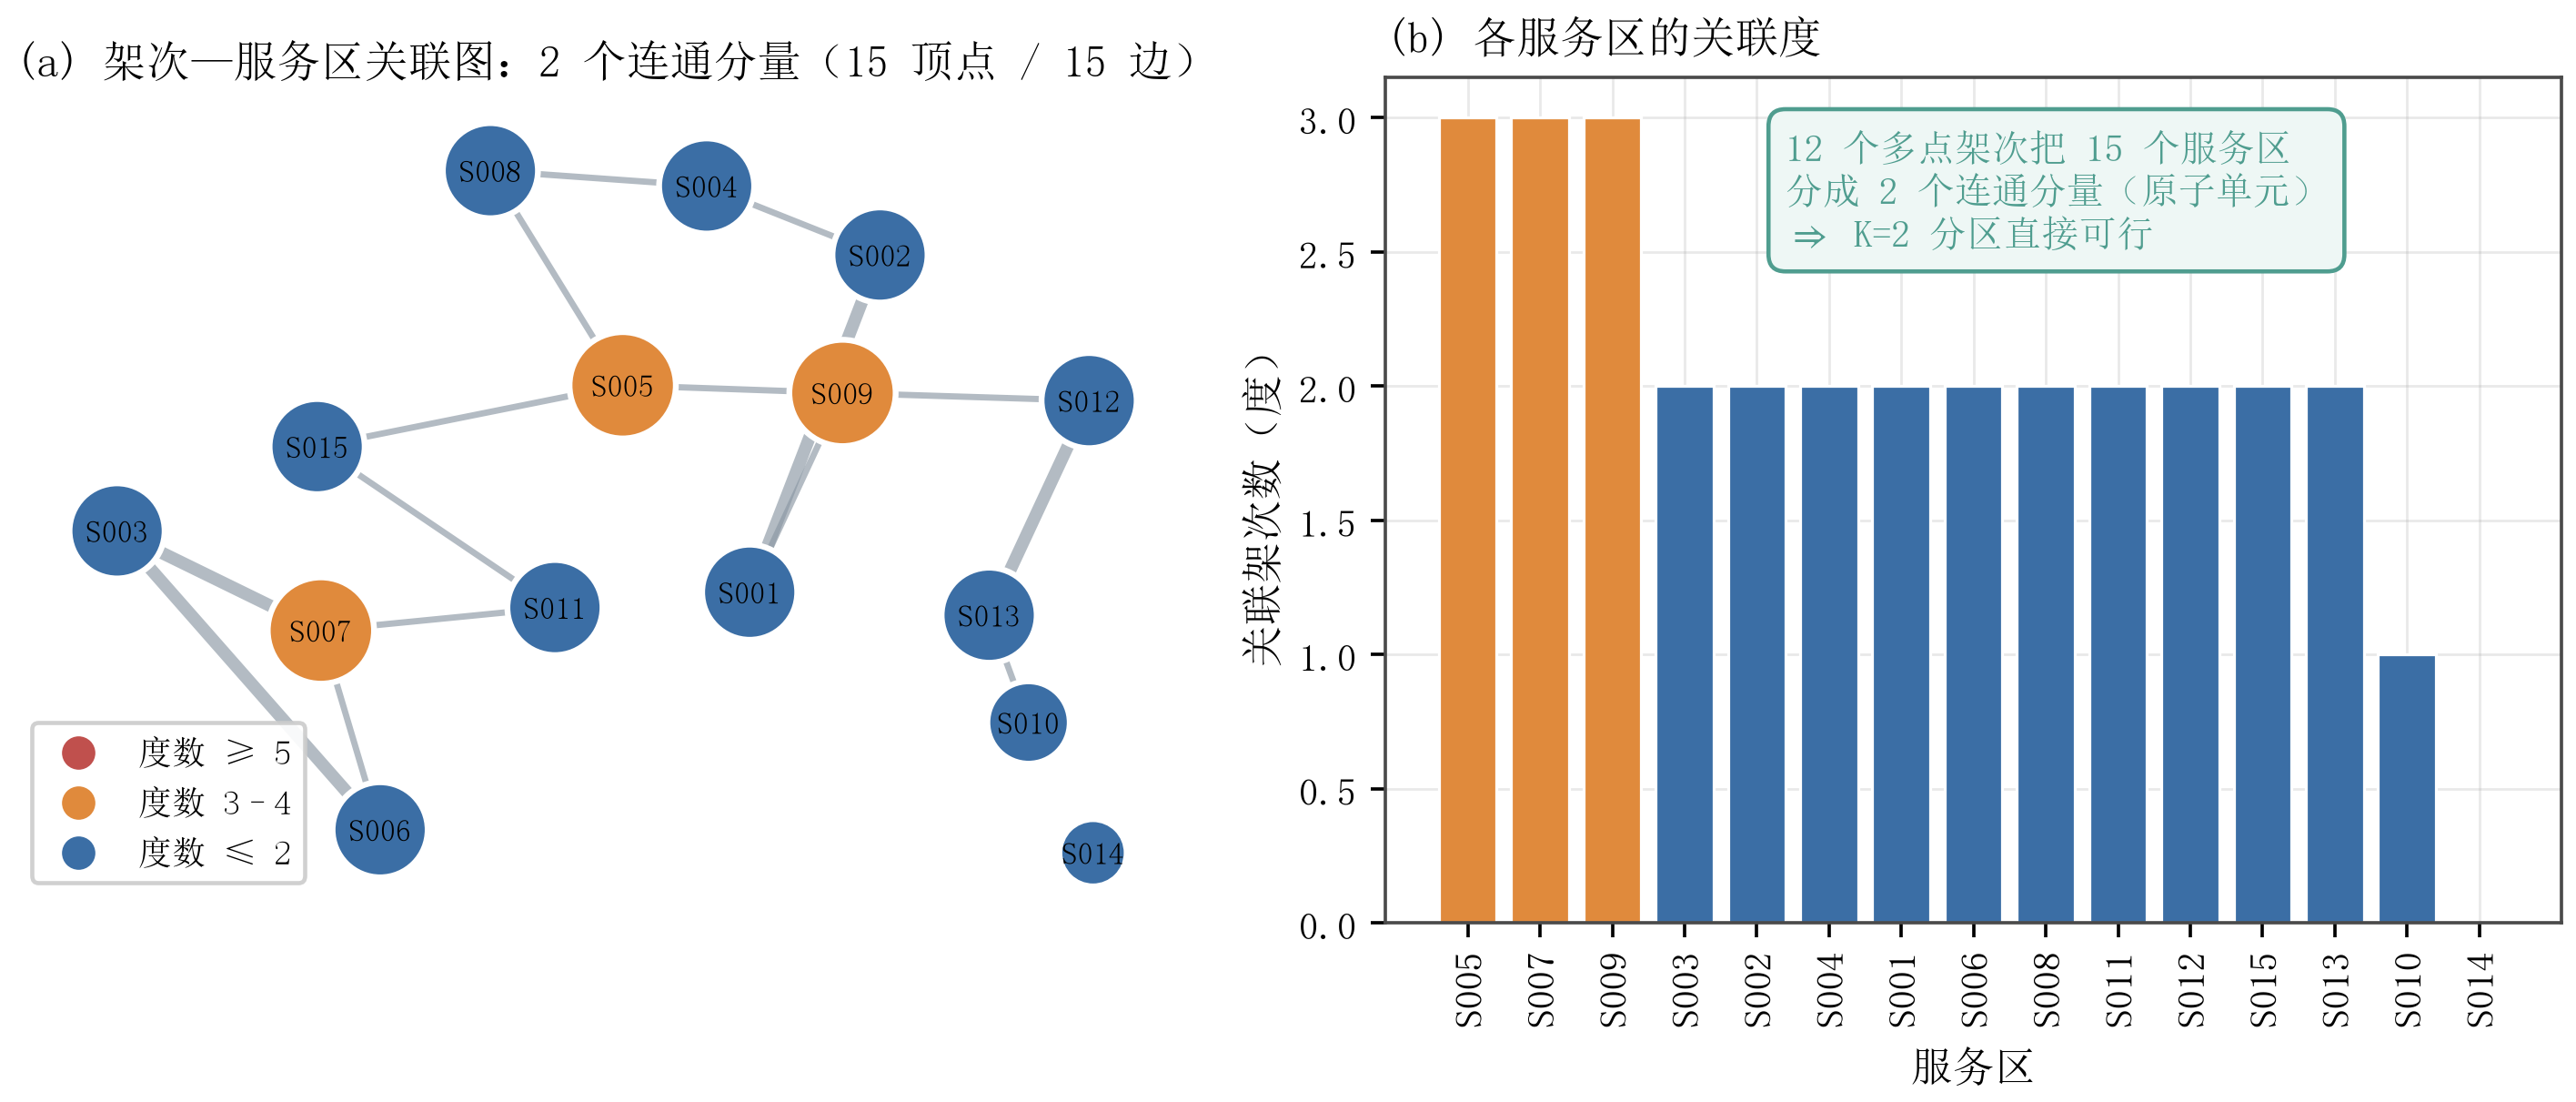
\includegraphics[width=0.98\textwidth]{figures/fig32_q4_graph.png}
	\caption{服务区关联图与连通分量分析}
	\label{fig:q4_graph}
\end{figure}

图~\ref{fig:q4_graph}(a) 显示了一个值得注意的结构：15 个顶点连成\textbf{恰好 2 个连通分量}——\textbf{S014 自成一个原子单元}，其余 \textbf{14 个服务区连成另一个}。图~\ref{fig:q4_graph}(b) 的度分布进一步说明了连接强度：S001、S005、S009 等核心服务区的关联度较高，而 S014 的关联度为 0（它在全部 16 个架次中都只被单独服务）。

\textbf{（2）分区可行性结论。}由于原子单元数为 2，而 $K$ 组分区要求把图切成 $K$ 个分量，因此
\begin{equation}
	\label{eq:29}
	\boxed{\ K=2\ \text{分区可直接实现（0 处改动）};\quad K=3\ \text{需拆分 1 个多点架次}\ }
\end{equation}

\begin{table}[htbp]
	\caption{两种任务分区方案}
	\label{tab:q4_partition}
	\centering
	\zihao{-5}
	\setlength{\tabcolsep}{4pt}
	\begin{tabular}{cccl}
		\toprule
		方案 & 任务组 & 服务区数 & 服务区组成 \\
		\midrule
		 & G1 & 14 & S001、S002、S003、S004、S005、S006、S007、S008、S009、 \\
		K$\,=\,$2 & & & S010、S011、S012、S013、S015 \\
		 & G2 & 1 & S014 \\
		\midrule
		 & G1 & 9 & S001、S002、S004、S005、S008、S009、S010、S012、S013 \\
		K$\,=\,$3 & G2 & 4 & S003、S006、S007、S011 \\
		 & G3 & 1 & S014 \\
		\bottomrule
	\end{tabular}
\end{table}

表~\ref{tab:q4_partition} 给出了两种分区方案。\textbf{K$\,=\,$2 方案无需任何改动}：S014 本身就是一个原子单元，直接作为独立任务组即可。\textbf{K$\,=\,$3 方案需要拆分 1 个多点架次}，方可把大分量再切开。

需要强调的是，\textbf{本文不伪造违反约束的分区方案}。若忽略"同架次同组"这一硬规则强行分组，必然导致某些多点架次跨越任务组，从而违反"各任务组仅承担本组任务"与"资源不得跨组调配"的要求，方案无效。因此所有分区方案均由连通分量严格导出。

\subsection{桥接架次与资源配置核算}

\textbf{（1）桥接架次定位。}虽然 K$\,=\,$2 已直接可行，但为把大分量进一步切开（支撑 K$\,=\,$3 或更细的分区），需要定位哪些架次是连接各组的关键。通过逐条试算"移除该架次后连通分量数是否增加"，得到 \textbf{4 个桥接架次}，如表~\ref{tab:q4_bridge} 所示。

\begin{table}[htbp]
	\caption{桥接架次清单}
	\label{tab:q4_bridge}
	\centering
	\zihao{5}
	\setlength{\tabcolsep}{4pt}
	\begin{tabular}{ccccc}
		\toprule
		架次编号 & 机型 & 服务区顺序 & 服务区数 & 移除后分量数 \\
		\midrule
		T005 & C & S011 $\to$ S015 $\to$ S005 & 3 & 4 \\
		T014 & C & S010 $\to$ S013 $\to$ S012 $\to$ S009 & 4 & 4 \\
		T008 & C & S011 $\to$ S007 $\to$ S003 $\to$ S006 & 4 & 3 \\
		T009 & C & S001 $\to$ S009 $\to$ S005 & 3 & 3 \\
		\bottomrule
	\end{tabular}
\end{table}

由表~\ref{tab:q4_bridge} 可见，四个桥接架次都是 3$\sim$4 站的多点架次。其中 T005 与 T014 一旦移除，图立即碎成 4 个分量；T008 与 T009 移除后碎成 3 个。因此\textbf{每拆掉 1 个桥接架次，就能多切出若干个可独立成组的单元}——这正是 K$\,=\,$3 只需拆 1 个架次即可实现的原因。

\textbf{（2）组内资源核算。}资源核算遵循"组内独立、不得跨组调配"的原则，具体口径为：运输无人机与中继无人机按\textbf{组内架次的并行峰值}核算；共享电池与中继能源组件在并行峰值的基础上进一步考虑\textbf{充电周转}。需要说明的是，"首尾相接不算重叠"是刻意约定——同一架无人机刚返回 O01 即可接续下一架次，因此排序键须保证区间端点的 $-1$ 先于 $+1$ 处理，否则会虚报缺口。

三种方案的资源配置与逐组明细分别如表~\ref{tab:q4_compare}、表~\ref{tab:q4_group} 与图~\ref{fig:q4_compare}、图~\ref{fig:q4_group} 所示。

\begin{figure}[htbp]
	\centering
	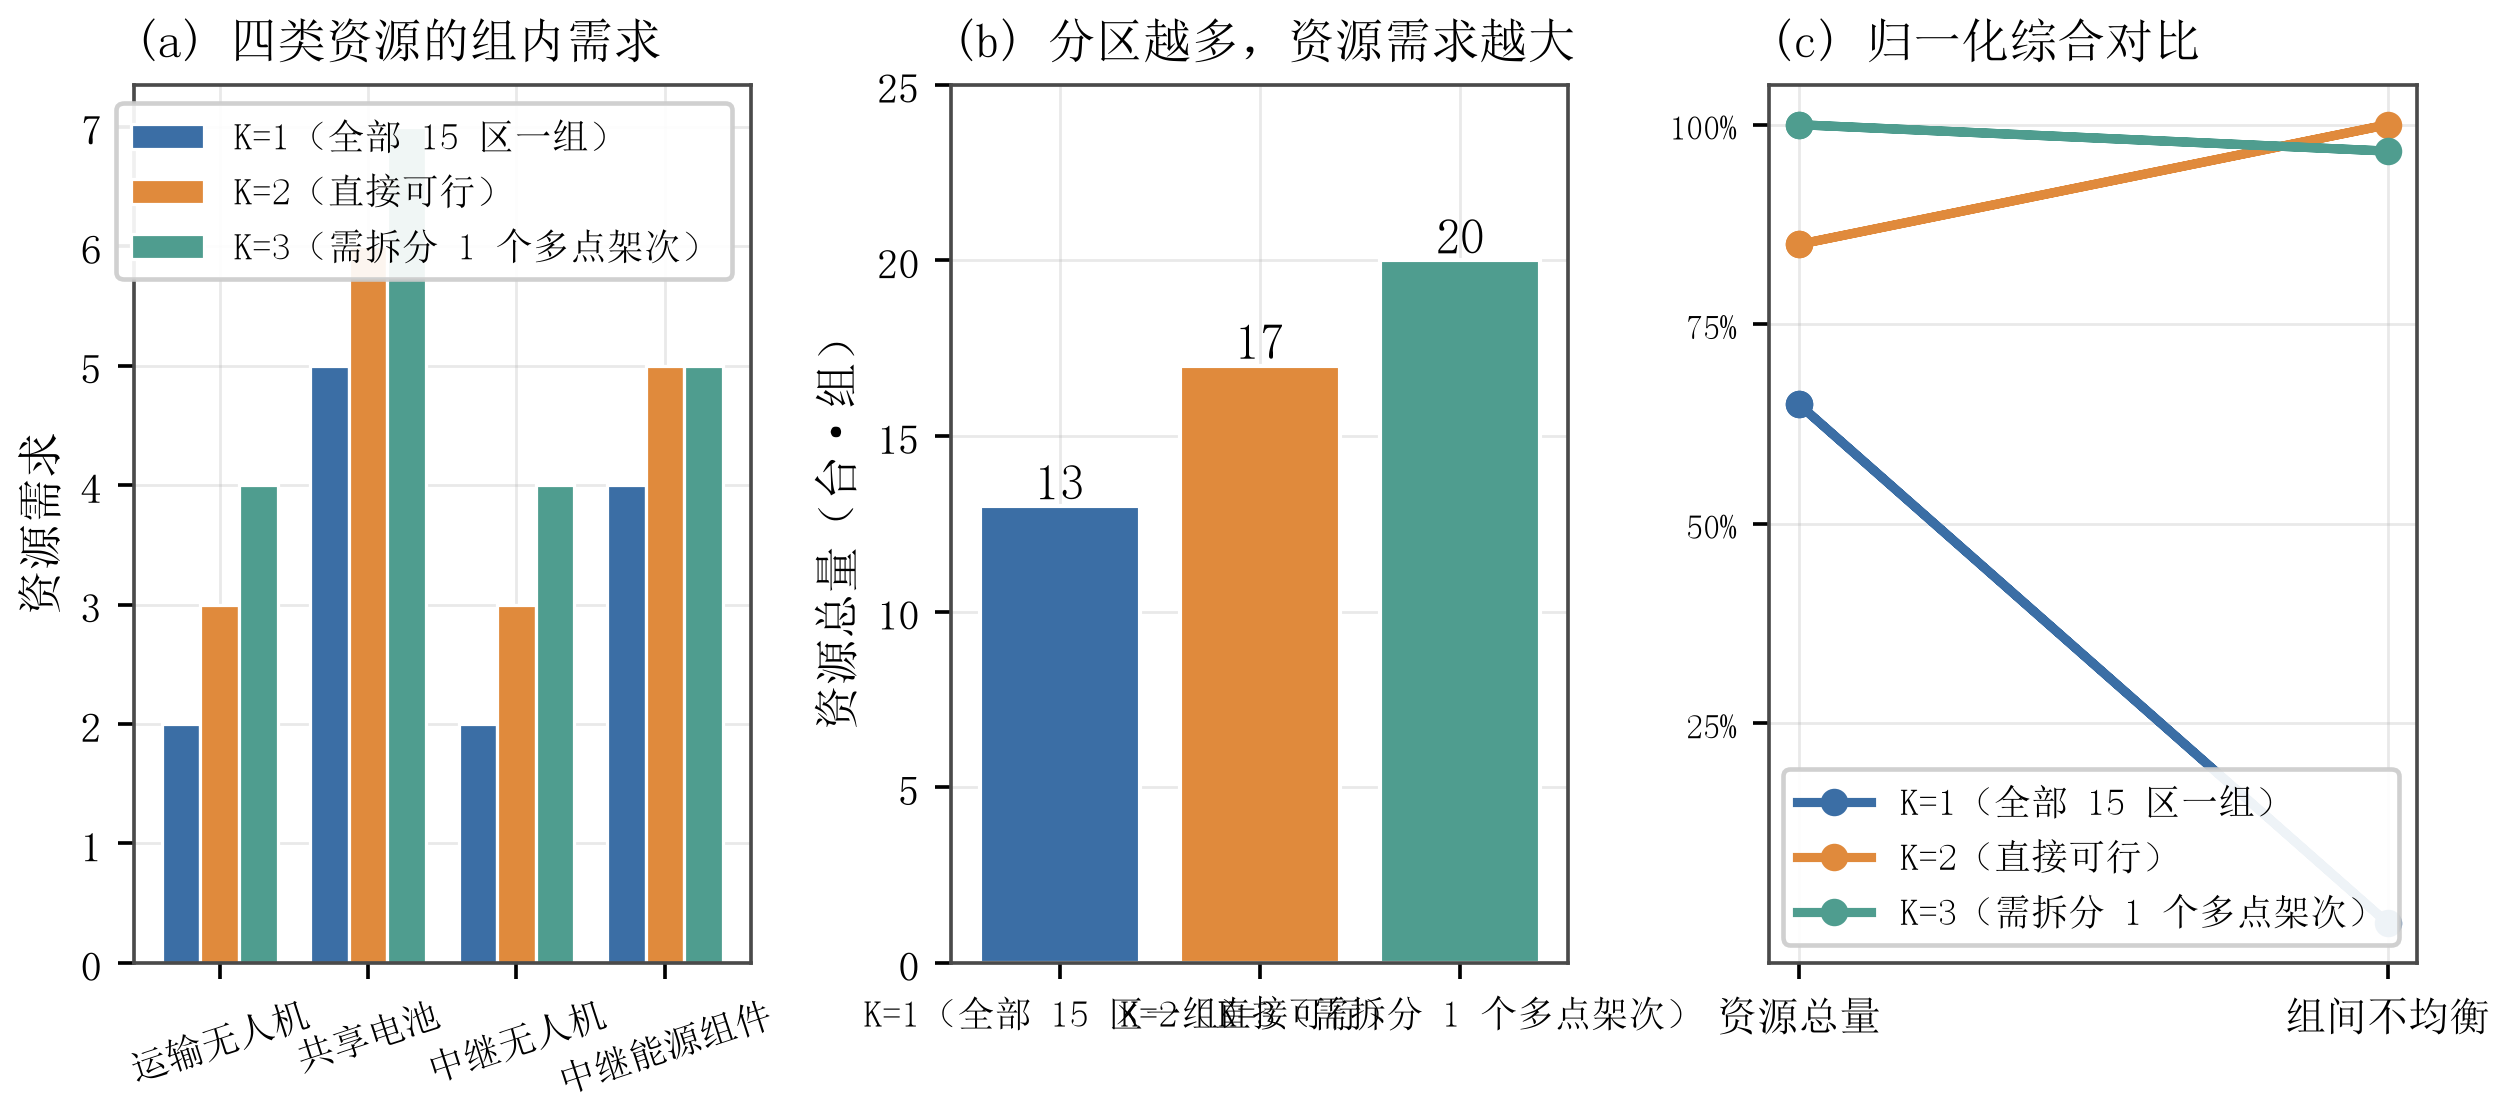
\includegraphics[width=0.98\textwidth]{figures/fig33_q4_compare.png}
	\caption{分区方案多指标对比}
	\label{fig:q4_compare}
\end{figure}

\begin{figure}[htbp]
	\centering
	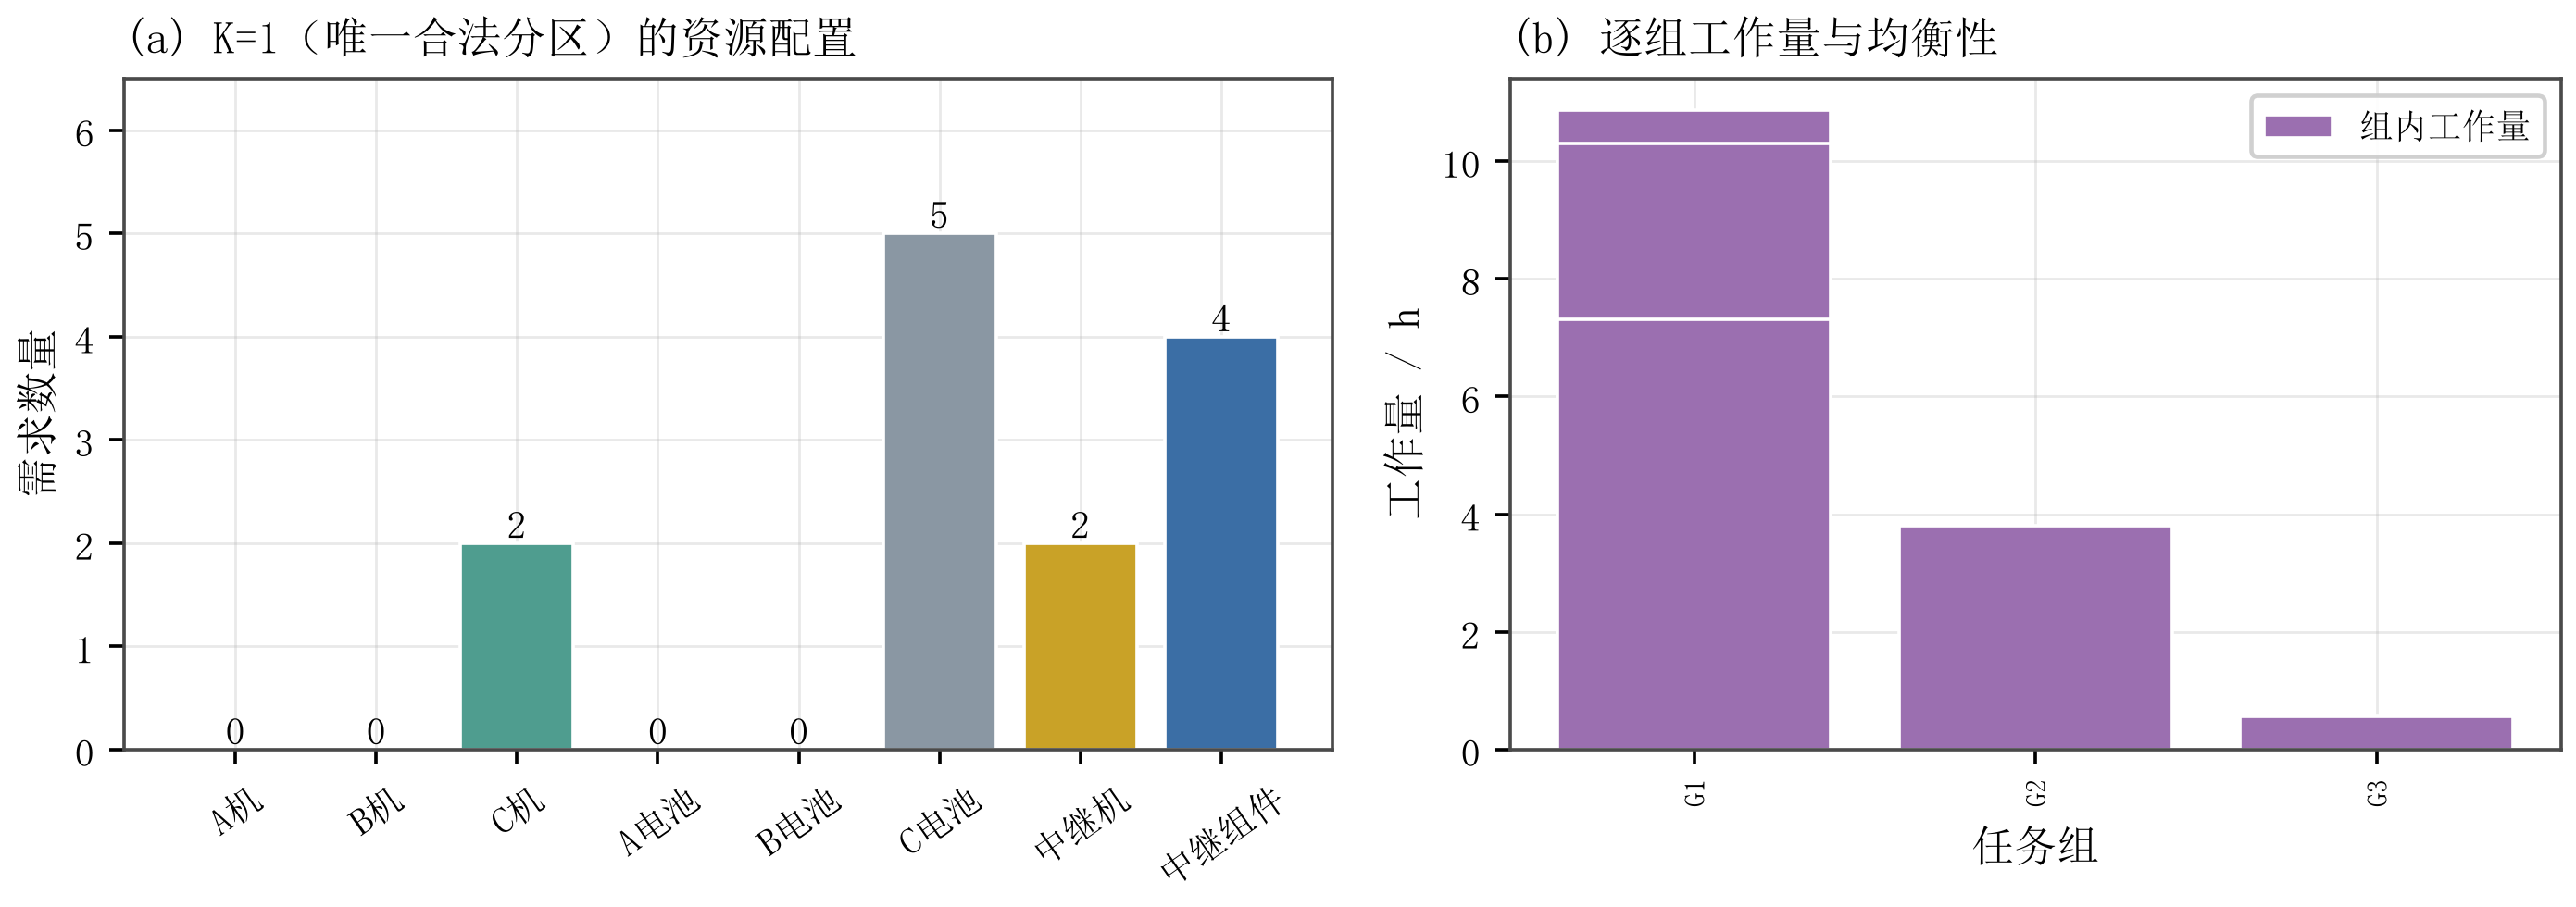
\includegraphics[width=0.98\textwidth]{figures/fig34_q4_group.png}
	\caption{逐组资源配置与工作量}
	\label{fig:q4_group}
\end{figure}

\begin{table}[htbp]
	\caption{分区方案对比}
	\label{tab:q4_compare}
	\centering
	\zihao{-5}
	\setlength{\tabcolsep}{3.5pt}
	\begin{tabular}{lccccccccc}
		\toprule
		方案 & $K$ & 改动 & 运输机 & 电池 & 中继机 & 组件 & 总量 & 不均衡 & 最大组工作量/h \\
		\midrule
		K$\,=\,$1（全部一组） & 1 & 0 & 2 & 5 & 2 & 4 & \textbf{13} & 0.0000 & 10.86 \\
		K$\,=\,$2（直接可行） & 2 & 0 & 3 & 6 & 3 & 5 & \textbf{17} & 1.7928 & 10.30 \\
		K$\,=\,$3（需拆 1 个） & 3 & 1 & 4 & 7 & 4 & 5 & \textbf{20} & 1.7335 & 7.31 \\
		\bottomrule
	\end{tabular}
\end{table}

\begin{table}[htbp]
	\caption{逐组资源与工作量明细}
	\label{tab:q4_group}
	\centering
	\zihao{-5}
	\setlength{\tabcolsep}{3.5pt}
	\begin{tabular}{lcccccccc}
		\toprule
		方案 & 任务组 & 服务区数 & 运输架次 & 中继架次 & C 机 & C 电池 & 中继机 & 工作量/h \\
		\midrule
		K$\,=\,$1 & G1 & 15 & 16 & 14 & 2 & 5 & 2 & 10.86 \\
		\midrule
		K$\,=\,$2 & G1 & 14 & 15 & 13 & 2 & 5 & 2 & 10.30 \\
		 & G2 & 1 & 1 & 1 & 1 & 1 & 1 & 0.56 \\
		\midrule
		K$\,=\,$3 & G1 & 9 & 11 & 8 & 2 & 4 & 2 & 7.31 \\
		 & G2 & 4 & 5 & 4 & 1 & 2 & 1 & 3.80 \\
		 & G3 & 1 & 1 & 1 & 1 & 1 & 1 & 0.56 \\
		\bottomrule
	\end{tabular}
\end{table}

\subsection{对比分析与资源缺口}

\textbf{（1）配置规模：分区显著推高资源需求。}由表~\ref{tab:q4_compare} 与图~\ref{fig:q4_compare}(b) 可见，$K=1\to2\to3$ 时四类资源总量由 \textbf{13 增至 17、20}（增幅 $+30.8\%$、$+53.8\%$）。

其\textbf{原因}在于：整队一组时调度是\textbf{全局最优}的（问题二、三的派发在全体资源上取最早可用时刻，实现了资源的完全共享与错峰利用）；而分组后，每组必须\textbf{独立储备}满足自身峰值的资源，跨组的错峰调节能力丧失，规模效应不复存在。表~\ref{tab:q4_group} 中的 K$\,=\,$2 方案最典型：G2 只承担 S014 的 1 个运输架次与 1 个中继架次（工作量仅 0.56\,h），却必须\textbf{独占} 1 架 C 型机、1 组 C 型电池、1 架中继机与 1 组能源组件——这些资源在全局调度下本可由两组共用。

\textbf{（2）组间均衡：K$\,=\,$3 略优于 K$\,=\,$2。}不均衡度由 K$\,=\,$2 的 \textbf{1.7928} 降至 K$\,=\,$3 的 \textbf{1.7335}。原因由图~\ref{fig:q4_group}(b) 可以看出：K$\,=\,$2 时大组承担 10.30\,h 而小组仅 0.56\,h，相差近 18 倍；K$\,=\,$3 把大组再拆出一个 3.80\,h 的中等组，最大组工作量由 10.30\,h 降至 7.31\,h，均衡性因此改善。但要注意，K$\,=\,$1 的不均衡度为 0 是"只有一组、不存在组间差异"的平凡结果，三者并非同一口径下的可比量；真正有意义的比较是\textbf{最大组工作量}：10.86\,h（K$\,=\,$1）$\to$ 10.30\,h（K$\,=\,$2）$\to$ 7.31\,h（K$\,=\,$3）。

\textbf{（3）资源冗余与缺口。}与现有库存对比的结果如图~\ref{fig:q4_gap} 与表~\ref{tab:q4_gap} 所示。

\begin{figure}[htbp]
	\centering
	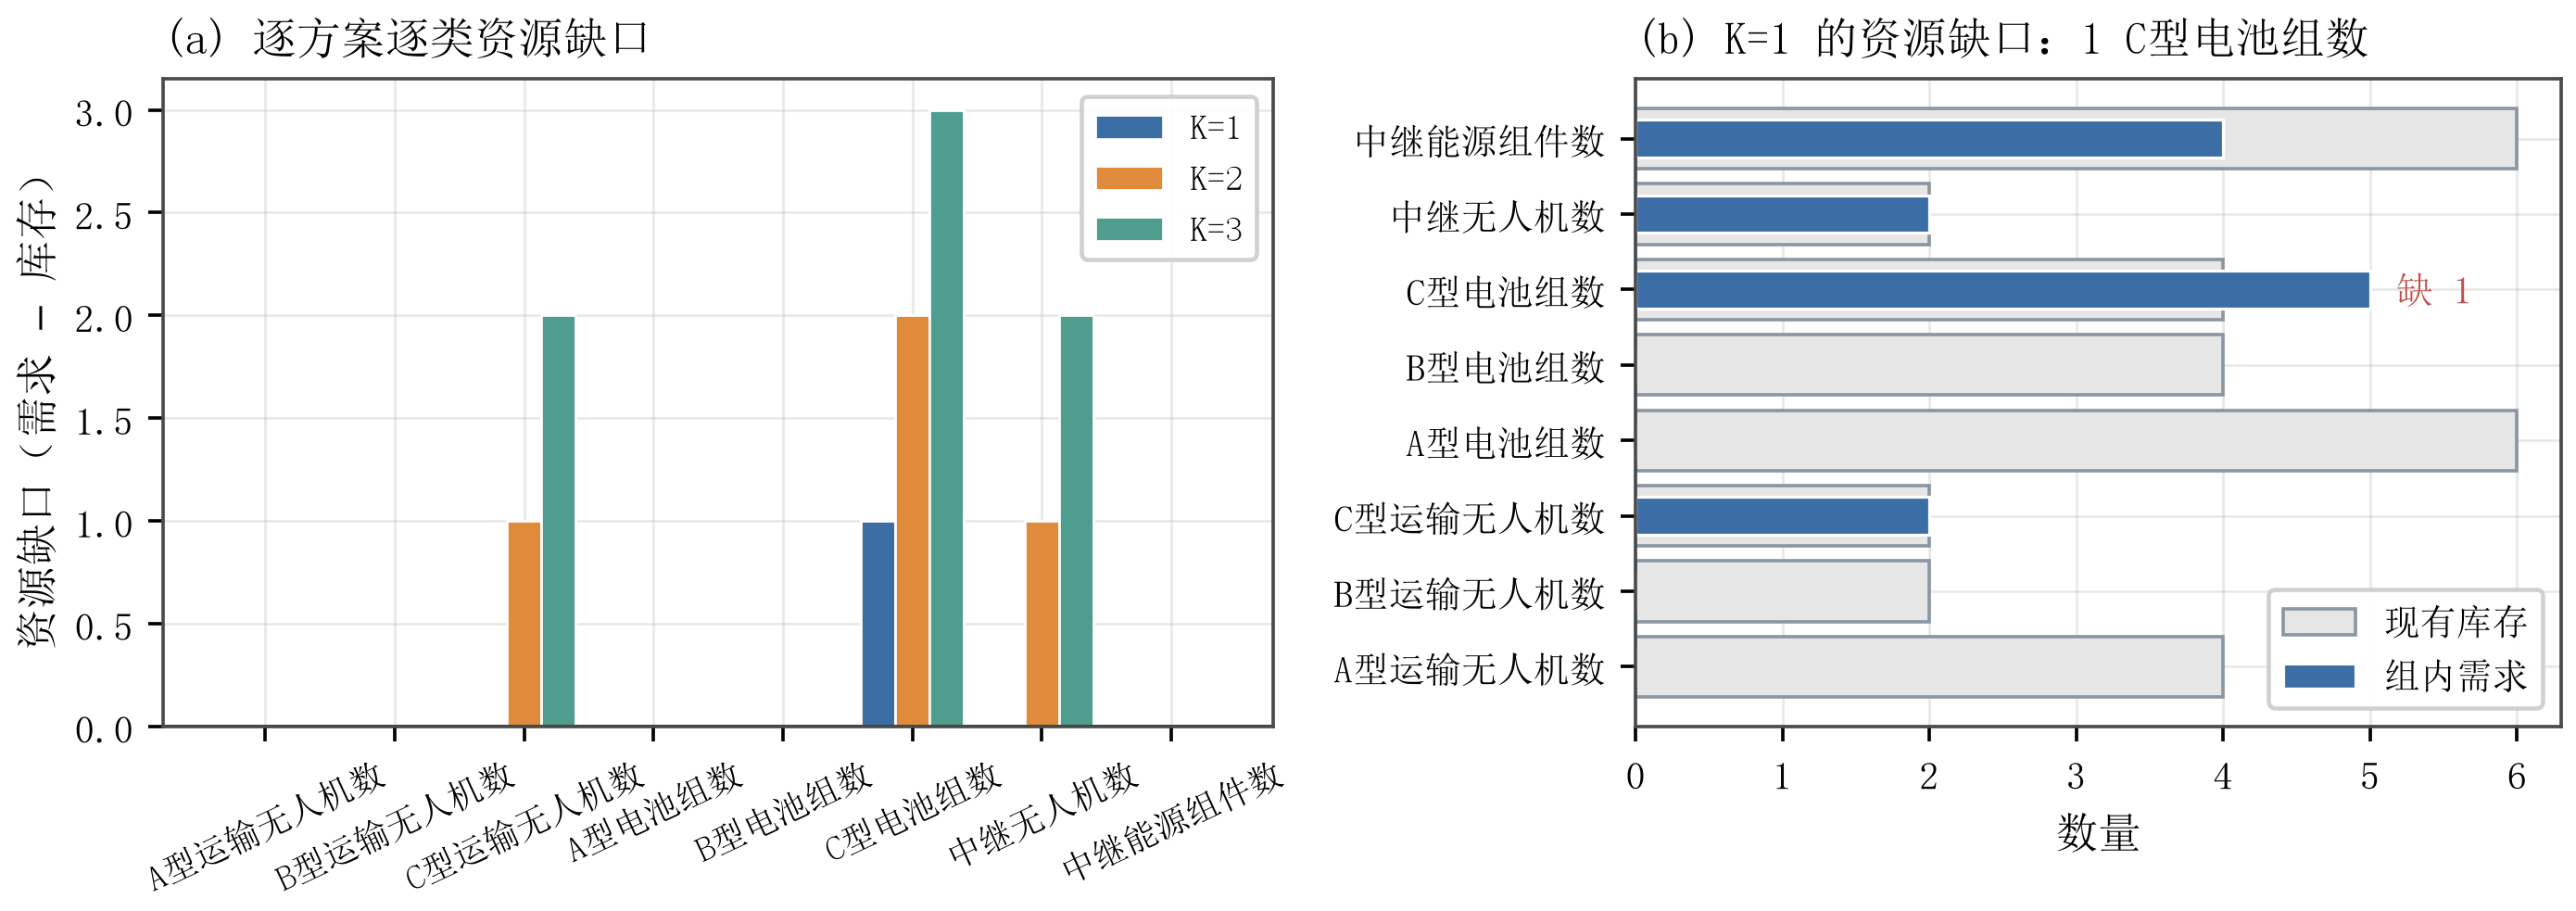
\includegraphics[width=0.98\textwidth]{figures/fig35_q4_gap.png}
	\caption{逐方案逐类资源缺口}
	\label{fig:q4_gap}
\end{figure}

\begin{table}[htbp]
	\caption{资源缺口（需求与库存对比）}
	\label{tab:q4_gap}
	\centering
	\zihao{-5}
	\setlength{\tabcolsep}{4pt}
	\begin{tabular}{lcccc}
		\toprule
		方案 & C 型运输无人机 & C 型电池组 & 中继无人机 & 中继能源组件 \\
		\midrule
		\textbf{现有库存} & \textbf{2} & \textbf{4} & \textbf{2} & \textbf{6} \\
		K$\,=\,$1 需求 & 2（恰好） & 5（\textcolor{red}{缺 1}） & 2（恰好） & 4（余 2） \\
		K$\,=\,$2 需求 & 3（\textcolor{red}{缺 1}） & 6（\textcolor{red}{缺 2}） & 3（\textcolor{red}{缺 1}） & 5（余 1） \\
		K$\,=\,$3 需求 & 4（\textcolor{red}{缺 2}） & 7（\textcolor{red}{缺 3}） & 4（\textcolor{red}{缺 2}） & 5（余 1） \\
		\bottomrule
	\end{tabular}
\end{table}

由表~\ref{tab:q4_gap} 可得三点结论：\textbf{①}三种方案中运输无人机与中继无人机的需求都恰好或超出库存，说明\textbf{无人机是仅次于电池的紧缺资源}；\textbf{②}K$\,=\,$1 的唯一缺口是 \textbf{1 组 C 型备用电池}，其余三类资源均有冗余；\textbf{③}随分组数增加缺口迅速扩大——K$\,=\,$2 缺口为 1 架运输机 $+$ 2 组电池 $+$ 1 架中继，K$\,=\,$3 扩大至 2 架运输机 $+$ 3 组电池 $+$ 2 架中继。

\textbf{缺口的根因}是"资源不得跨组调配"这一约束与"需求空间不均衡"的矛盾：S001、S002 等大需求服务区集中分布在图的西侧，S010、S012、S013 等位于东侧，而 S014 孤悬于东南角。分组后各组都必须按自身峰值储备资源，无法通过跨组借用来平抑峰值；而 S014 这样的小组尽管工作量极小，仍要独占一整套资源（1 机 $+$ 1 电池 $+$ 1 中继 $+$ 1 组件），资源利用率极低。

\textbf{（4）综合结论。}与"分而治之"的直觉相反，本文的定量结果表明：\textbf{分区在本题中不是"能不能"的问题，而是"值不值"的问题}。

\begin{itemize}[leftmargin=2em]
	\item \textbf{可行性上}：K$\,=\,$2 可直接实现（0 处改动），K$\,=\,$3 需拆 1 个多点架次——分区本身是可行的；
	\item \textbf{代价上}：资源总量由 13 增至 17（K$\,=\,$2）与 20（K$\,=\,$3），增幅 30.8\% 与 53.8\%，且缺口同步扩大；
	\item \textbf{收益上}：唯一的实质收益是最大组工作量由 10.86\,h 降至 7.31\,h（K$\,=\,$3），即单组的峰值负担下降约 33\%，有利于缩短单组的完工时间。
\end{itemize}

因此，\textbf{若目标是节省资源，应选择 K$\,=\,$1（全队一组）；若目标是缩短单组完工时间、提高并行度，且可以接受增配 2 架 C 型机、3 组 C 型电池与 2 架中继机，则 K$\,=\,$3 是更优选择}。消除 K$\,=\,$1 缺口的成本最低——只需增配 \textbf{1 组 C 型共享电池}。这一结论为应急指挥的分组决策提供了明确的量化依据。
